\section{Description of the Project}
Our goal for this project is to visualize word embeddings by avoiding the clutters caused by too many data points. 
Our core idea for the approach is to cluster the data points and annotate with something that correctly summerizes the cluster. 
Figure~\ref{fig:cluster_network} shows the example output of our visualization. 

\begin{figure}[htb]
 \centering
     {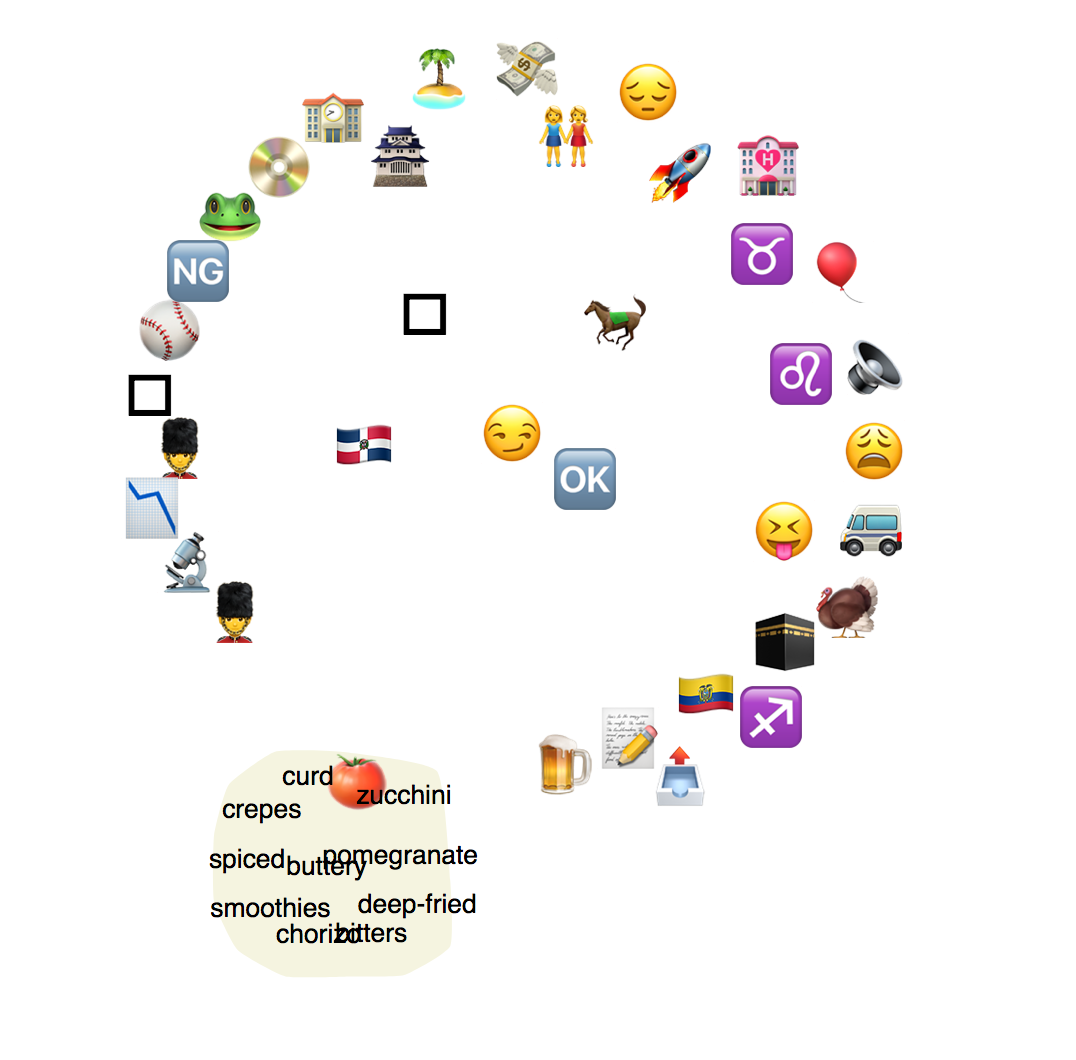
\includegraphics[width=0.68\linewidth]{figures/clustered_network.png}}
    \vspace{-1ex}
     \caption{The visualizaiton of word embeddings using clustered network and emojis.}
\label{fig:cluster_network}
\end{figure}

\begin{figure}[htb]
 \centering
     {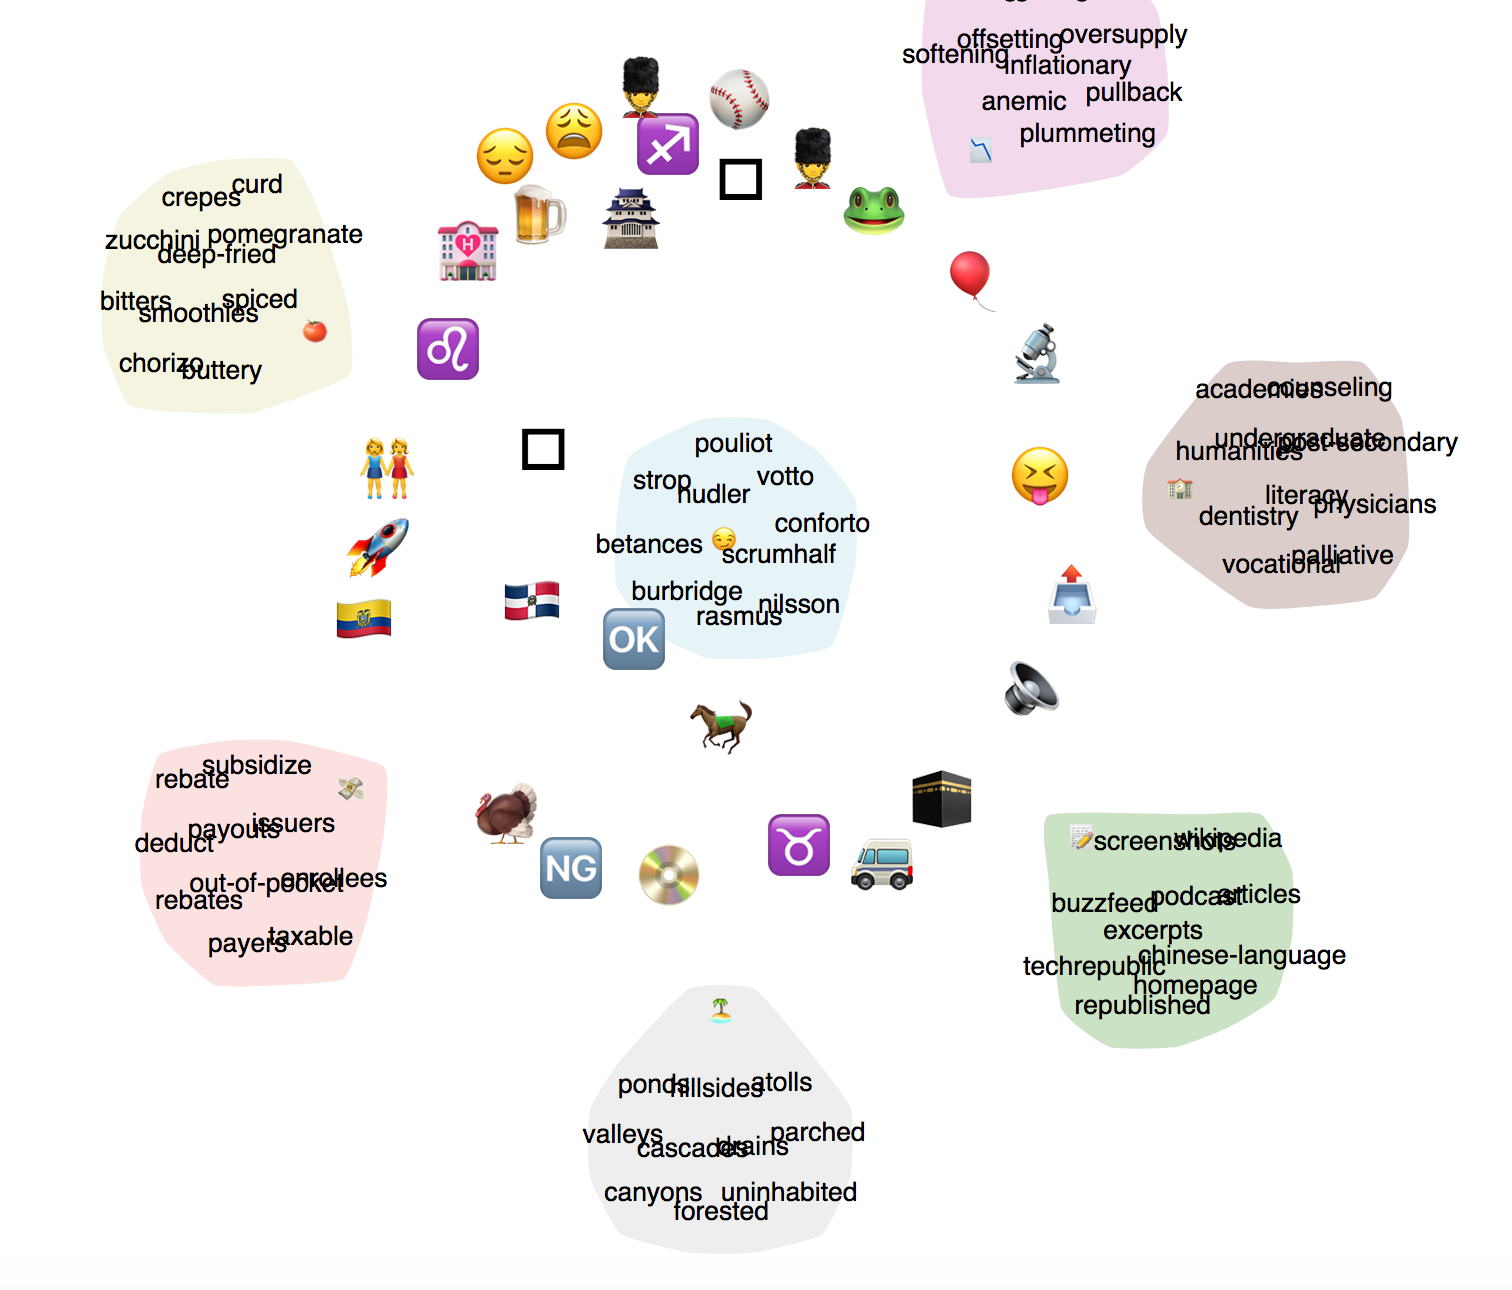
\includegraphics[width=0.68\linewidth]{figures/clustered_network_opened.png}}
    \vspace{-1ex}
     \caption{The visualizaiton of word embeddings using clustered network and emojis.}
\label{fig:cluster_network_opened}
\end{figure}

Our approach for constructing the visualization is as follows:
\begin{enumerate}
 \item Train a word embedding using a raw corpus. 
 \item Run $k$-means \cite{lloyd1982least} and obtain clusters
 \item Assign an emoji to each cluster
 \item Visualize using D3.js
\end{enumerate}
For the number of clusters $k$, we empirically set $k = \{40, 50\}$.

\subsection{Annotation of Clusters with Emojis}
When a human look at emoji, one connects with various possible concepts. 
Searching for a right word to represent the cluster requires external linguistic resources e.g., WordNet. 
However, images does not associate a single word. 
For example, when one looks at 🍅, the possible association of this words are ``tomato'', ``vegatable'', ``food'', or even ``object''. 
Therefore, we decide to use emojis to represent the clusters. 

Another motivation of using emojis instead of words is the ``Picture superiority effect'' (e.g., \cite{doi:10.1162/jocn.2010.21464}) i.e., humans are better remembering pictures than words. 
Assuming that the annotation of clusters is the most cruicial component of this visualization, we use emojis to represent the clusters.  

To assign an optimal emoji $e_c$ to each cluster $c$ with centroid vector $v_c$, assume we have a set of emoji and its text description $t$. 
We compute the mean word vector $v_t$ of each word $w_i$ in a given emoji description $t = \{w_1, w_2, ..., w_n\}$ with length $n$ out of all set of emoji descriptions $T$, i.e.,
\begin{equation}
 e_c =  \text{argmax}_{t \in T} \text{cos\_sim}(v_c, v_t)
\end{equation}
where 
\begin{equation}
 v_t = \frac{\sum_{i = 1}^{n} w_i}{n}. 
\end{equation}

Word vectors are trained by Skip-gram with negative sampling \cite{NIPS2013_5021} using 1 million sentences of English news articles from Leipzig corpora collection \cite{Goldhahn12buildinglarge}. We set the word vector dimension as $100$. 
Emojis are obtained from dataset built by \cite{eisner-EtAl:2016:SocialNLP}. 


\subsection{Interaction}
Users can click on emojis to ``drill-down'' \cite{Elmqvist:2010:HAI:1749404.1749525} the cluster and look into the nearest neighboring words in terms of the centroid in the cluster.

\subsection{Force Layout}
To solve the problem of overlapping texts, we also use force layout in D3.js to let the texts and emojis move and draggable. 
